\section{Discussion}
\subsection{Σύγκριση Fitness vs Imitation Dynamics}
	\begin{figure}[h]
	      \centering
	      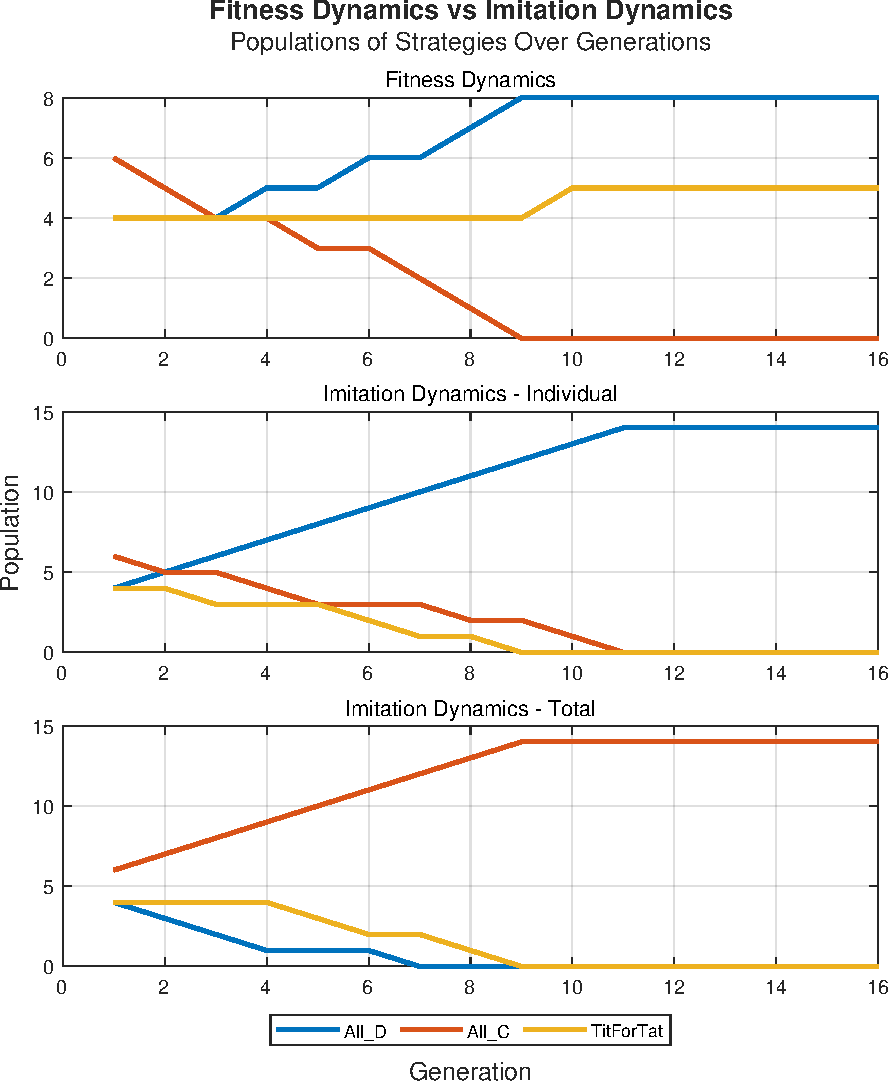
\includegraphics[width=0.9\textwidth]{Fitness Dynamics vs Imitation Dynamics.pdf}
	      \caption{Fitness Dynamics vs Imitation Dynamics $\begin{bmatrix}All\_D&All\_C&TitForTat\end{bmatrix}$ $POP0=\begin{bmatrix}4&6&4\end{bmatrix}$}
	      \label{fig:Fitness Dynamics vs Imitation Dynamics}
	\end{figure}
Στο Σχήμα \ref{fig:Fitness Dynamics vs Imitation Dynamics} γίνεται μία σύγκριση μεταξύ των αποτελεσμάτων των TourSimFit, TourSimImi με mode=''Individual'' και TourSimImi με mode=''Total'' για στρατηγικές $\begin{bmatrix}All\_D&All\_C&TitForTat\end{bmatrix}$ με $POP0=\begin{bmatrix}4&6&4\end{bmatrix}$.
Παρατηρούμε ότι η περίπτωση Fitness μοιάζει με την περίπτωση ``Individual'' mode, ωστόσο και μεταξύ των δύο σημειώνεται η σημαντική διαφορά ότι στα Imitation Dynamics επιβιώνει μόνο μία στρατηγική. Η περίπτωση του ``Total'' mode έχει παρόμοια εξέλιξη με το ``Individual'' mode αλλά παρατηρούμε ότι επιβιώνει διαφορετική στρατηγική, συγκεκριμένα η ``All\_C'', επειδή έχει αρχικό πληθυσμό μεγαλύτερο από τις άλλες στρατηγικές και άρα εκμεταλλεύεται καλύτερα την συμπαθή στρατηγική ``TitForTat'' μέσω της λειτουργίας του ``Total'' mode για εύρεση της βέλτιστης στρατηγικής.

\subsection{Τελικά Συμπεράσματα}
Από την παραπάνω ανάλυση των δύο εξελικτικών δυναμικών προκύπτουν τα παρακάτω συμπεράσματα:

\subsubsection*{Για τα Fitness Dynamics}
α) Οι Mathieu et al φαίνεται ότι χρησιμοποιούσαν απλό floor κατά τον υπολογισμό των νέων πληθυσμών μετά από κάθε γενιά, καθώς η τακτική αυτή δημιούργησε για εμάς τα κοντινότερα αποτελέσματα.

β) Σε πολλές περιπτώσεις ασταθών, γενικά, συμπεριφορών, τα διαγράμματα διαφοροποιούνται σε παρατηρήσιμο βαθμό ανάλογα με το αν χρησιμοποιείται η συνάρτηση TourTheFit ή η συνάρτηση TourSimFit με και χωρίς compensation. Αυτό οφείλεται στο ότι πολλές από τις περιπτώσεις των διαγραμμάτων που προκύπτουν είναι ιδιαίτερα ευαίσθητες και έτσι, ακόμα και μικρή μεταβολή στη λογική της δυναμικής, μπορεί να αλλάξει τα αποτελέσματα σημαντικά.

γ) Το διάγραμμα που προκύπτει εξαρτάται από τις αρχικές τιμές πληθυσμού, τις στρατηγικές που χρησιμοποιούνται και τον πίνακα απολαβής. Ακόμα και για 2 από αυτούς τους παράγοντες ίδιους, η μεταβολή ενός από αυτούς μπορεί να οδηγήσει σε δραστικά διαφορετικά αποτελέσματα (ακόμα και διαφορετική ταξινόμηση, όπως στην 5η προσομοίωση).

δ) Η ανάθεση των εναπομείναντων μελών του πληθυσμού τυχαία σύμφωνα με τη λογική του compensation φαίνεται να είναι καλή επιλογή, ειδικά σε σχέση με την απλότητά της, διότι δε μεταβάλλει σημαντικά τα αποτελέσματα (στρατηγικές που θεωρητικά πεθαίνουν, πεθαίνουν πραγματικά, γενικά το πού τείνουν οι πληθυσμοί δεν αλλάζει). Ανάλογα με την περίπτωση που εξετάζεται, μοιάζει περισσότερο είτε με την περίπτωση της TourTheFit είτε με την περίπτωση TourSimFit δίχως compensation.

ε) Σε γενικές γραμμές, η διακριτή φύση των προσομοιώσεων TourSimFit με ή χωρίς compensation, δημιουργεί σε βάθος χρόνου είτε επαναλαμβανόμενες ταλαντώσεις είτε σύγκλιση σε κάποιες τελικές τιμές πληθυσμού. Το χάος δεν μπορεί πραγματικά να επιτευχθεί, ακόμα και στην 6η προσομοίωση οι πληθυσμοί τελικά τείνουν στις τιμές που προβλέπει και η TourTheFit. Ωστόσο, αυτό δε μας αποτρέπει από το να δημιουργήσουμε τα ενδιαφέροντα αποτελέσματα που βλέπουμε και στο paper.

\subsubsection*{Για τα Imitation Dynamics}
α) Η επιλογή της ακριβής δυναμικής που ακολουθάται κατά τον υπολογισμό των πληθυσμών της επόμενης γενιάς είναι βασική για τα αποτελέσματα που προκύπτουν. Για παράδειγμα, η επιλογή K παικτών από τον συνολικό πληθυσμό ή K παικτών εκ των μη βέλτιστων, δημιουργούν πολύ διαφορετικά αποτελέσματα και θεωρητικά και στις προσομοιώσεις.

β) Οι περιπτώσεις υπολογισμού της βέλτιστης στρατηγικής με τη μέθοδο In\-di\-vi\-du\-al και Total οδηγούν επίσης σε δραστικά διαφορετικά αποτελέσματα για τη φύση των καταστάσεων που προκύπτουν, όπως φαίνεται στις προσομοιώσεις 2 και 3. Σε γενικές γραμμές, η μέθοδος Total δημιουργεί συνεκτικούς υπογράφους που έχουν ως τελικές καταστάσεις τις καταστάσεις επικράτησης μίας εκ των στρατηγικών, ενώ η μέθοδος Individual δημιουργεί έναν μεγαλύτερο υπογράφο που οδηγεί σε πολλές πιθανές τελικές καταστάσεις και μερικές απομονωμένες τελικές καταστάσεις. Ο όρος συνεκτικότητα χρησιμοποιείται εδώ λανθασμένα, καθώς πρόκειται για κατευθυνόμενους γράφους στους οποίους κατά κανόνα δεν υπάρχουν διαδρομές και προς τις δύο κατευθύνσεις, αλλά χρησιμοποιείται για τη χαλαρή επεξήγηση του φαινομένου.

γ) Λόγω του β), παρατηρούμε ότι η τελική κατάσταση δεν είναι πάντα βέβαιη γνωρίζοντας την αρχική, εφόσον επιλέγεται η μέθοδος Individual. Αυτό οφείλεται στο ότι η τυχαία ανάθεση ανά γενιά μπορεί να οδηγήσει διαφορετικές κάθε φορά στρατηγικές σε πλεονεκτική θέση την επόμενη γενιά, και άρα να υπάρχει μεταβλητότητα στα αποτελέσματα. Αντιθέτως, η μέθοδος Total είναι πλήρως ντετερμινιστική ως προς την αρχική και τελική κατάσταση, ενώ παρουσιάζει τυχαιότητα μόνο στο μονοπάτι που θα ακολουθηθεί μεταξύ των 2.

δ) Σε κάθε περίπτωση, οι πληθυσμοί που προκύπτουν από τη συνάρτηση Tour\-Sim\-Imi ακολουθούν κάποια σειρά μεταβολών που παρουσιάζεται στο διάγραμμα μετάβασης καταστάσεων της αντίστοιχης Tour\-The\-Imi και Analyze\-Markov\-Chain.
